\chapter{Cubed-sphere finite-volume methods}
\label{chp-cs-fv}

\section{Advection finite-volume scheme}
In this Chapter, we show how we can use the dimension splitting method
presented in Chapter \ref{chp-2d-fv} to solve the advection
equation on the cubed-sphere with base on \citet{putman:2007}.

We denote by $\Psi_p:[-a,a] \times [-a,a] \to \mathbb{S}^2_R$,
$p=1, \cdots, 6,$ as a cubed-sphere mapping introduce in Chapter \ref{chp-cs-grids}.
We introduce the notations:

\begin{itemize}
\item $(x,y;p)$ represents a point on the cubed-sphere using a cubed-sphere mapping;
\item $[-a,a]^2 = \bigcup_{i,j=1}^N [x_{i-\frac{1}{2}}, x_{i+\frac{1}{2}}] \times [y_{j-\frac{1}{2}}, y_{j+\frac{1}{2}}]$;
\item $\Delta x = x_{i+\frac{1}{2}}- x_{i-\frac{1}{2}},
\Delta y = y_{j+\frac{1}{2}}- y_{j-\frac{1}{2}}$;
\item $\Omega_{ijp} = \Psi_p([x_{i-\frac{1}{2}}, x_{i+\frac{1}{2}}] \times [y_{j-\frac{1}{2}}, y_{j+\frac{1}{2}}])$
are the cubed-sphere control-volumes;
\item
	$\boldsymbol{g}_{1}(x,y;p) = D\Psi_{p}(x,y)
	\begin{bmatrix}
		1 \\
		0
	\end{bmatrix} \text{and }
	\boldsymbol{g}_{2}(x,y;p) = D\Psi_{p}(x,y)
	\begin{bmatrix}
		0 \\
		1
	\end{bmatrix}
	$ are the tangent vectors;
\item
	$	g_{\Psi}(x,y) =
	\begin{bmatrix}
		\langle \boldsymbol{g}_{1}(x,y;p), \boldsymbol{g}_{1}(x,y;p) \rangle &
		\langle \boldsymbol{g}_{1}(x,y;p), \boldsymbol{g}_{2}(x,y;p) \rangle \\
		\langle \boldsymbol{g}_{1}(x,y;p), \boldsymbol{g}_{2}(x,y;p) \rangle  &
		\langle \boldsymbol{g}_{2}(x,y;p), \boldsymbol{g}_{2}(x,y;p) \rangle
	\end{bmatrix}
	$ is the metric tensor;
\item $\sqrt{\det{g_{\Psi}(x,y) }}$ is the metric tensor Jacobian;
\item $$|\Omega_{ijp}| = \int_{x_{i-\frac{1}{2}}}^{x_{i+\frac{1}{2}}} \int_{y_{i-\frac{1}{2}}}^{y_{i+\frac{1}{2}}}\sqrt{\det{g_{\Psi}(x,y) }} \,dx \,dy$$ are the control-volume areas

\item $$Q_{ijp}(t) = \frac{1}{|\Omega_{ijp}|}\int_{x_{i-\frac{1}{2}}}^{x_{i+\frac{1}{2}}}
\int_{y_{j-\frac{1}{2}}}^{y_{j+\frac{1}{2}}}  q(x,y,t;p) \sqrt{\det{g_{\Psi}(x,y) }}\,dx \,dy$$
are the averages of $q$ on the control-volumes;
\item $u_{i+\frac{1}{2},j,p}^n = u(x_{i+\frac{1}{2}},y_j,t_n;p);$
\item $v_{i,j+\frac{1}{2},p}^n = v(x_i,y_{j+\frac{1}{2}},t_n;p).$
\end{itemize}


Given a tangent velocity field $\boldsymbol{u}$ on the sphere, we denote its
contravariant components by $\tilde{u}$ and $\tilde{v}$.
For a give a detailed discussion on contravariant representations in Appendix \ref{anexo-sph}.
The advection equation on panel the $p$ of the cubed-sphere is given by:
\begin{equation*}
	\frac{\partial}{\partial t}{q}+
	\frac{1}{\sqrt{\det{g_{\Psi}}}}\bigg(
	\frac{\partial}{\partial x} {(\tilde{u}\sqrt{\det{g_{\Psi}}}q)}+
	\frac{\partial}{\partial y} {(\tilde{v}\sqrt{\det{g_{\Psi}}}q)}
	\bigg)
	= 0,
\end{equation*}
$\forall (x,y,t) \in [-a,a]^2\times[0,T]$, $q = {q}(x,y,t;p)$.
Its integral form is given by:
\begin{align*}
	{Q}_{ijp}(t_{n+1})  = {Q}_{ijp}(t_{n})
	&- \frac{\Delta t}{|\Omega_{ijp}|}
	\delta _x \bigg( \frac{1}{\Delta t}
	\int_{t_1}^{t_2} \int_{y_{j-\frac{1}{2}}}^{y_{j+\frac{1}{2}}}
	{(\tilde{u}\sqrt{\det{g_{\Psi}}}q)}(x_{i}, y, t;p)
	\,dy \,dt \bigg) \\ \nonumber
	&- \frac{\Delta t}{|\Omega_{ijp}|}
	\delta _y \bigg( \frac{1}{\Delta t}
	\int_{t_1}^{t_2} \int_{x_{i-\frac{1}{2}}}^{x_{i+\frac{1}{2}}}
	{(\tilde{v}\sqrt{\det{g_{\Psi}}}q)}(x, y_{j}, t;p)
	\,dx \,dt \bigg),
\end{align*}
Hence, we can use the dimension splitting presented in Chapter \ref{chp-2d-fv}
to the variable $\sqrt{\det{g_{\Psi}}}q$.
However, when computing the stencils near to the cube edges,
we need to approximate the values of $q$ in the ghost cells in order to compute
the stencils.


\begin{figure}[ht] % [H] é obrigatório em apresentações!
	\centering
	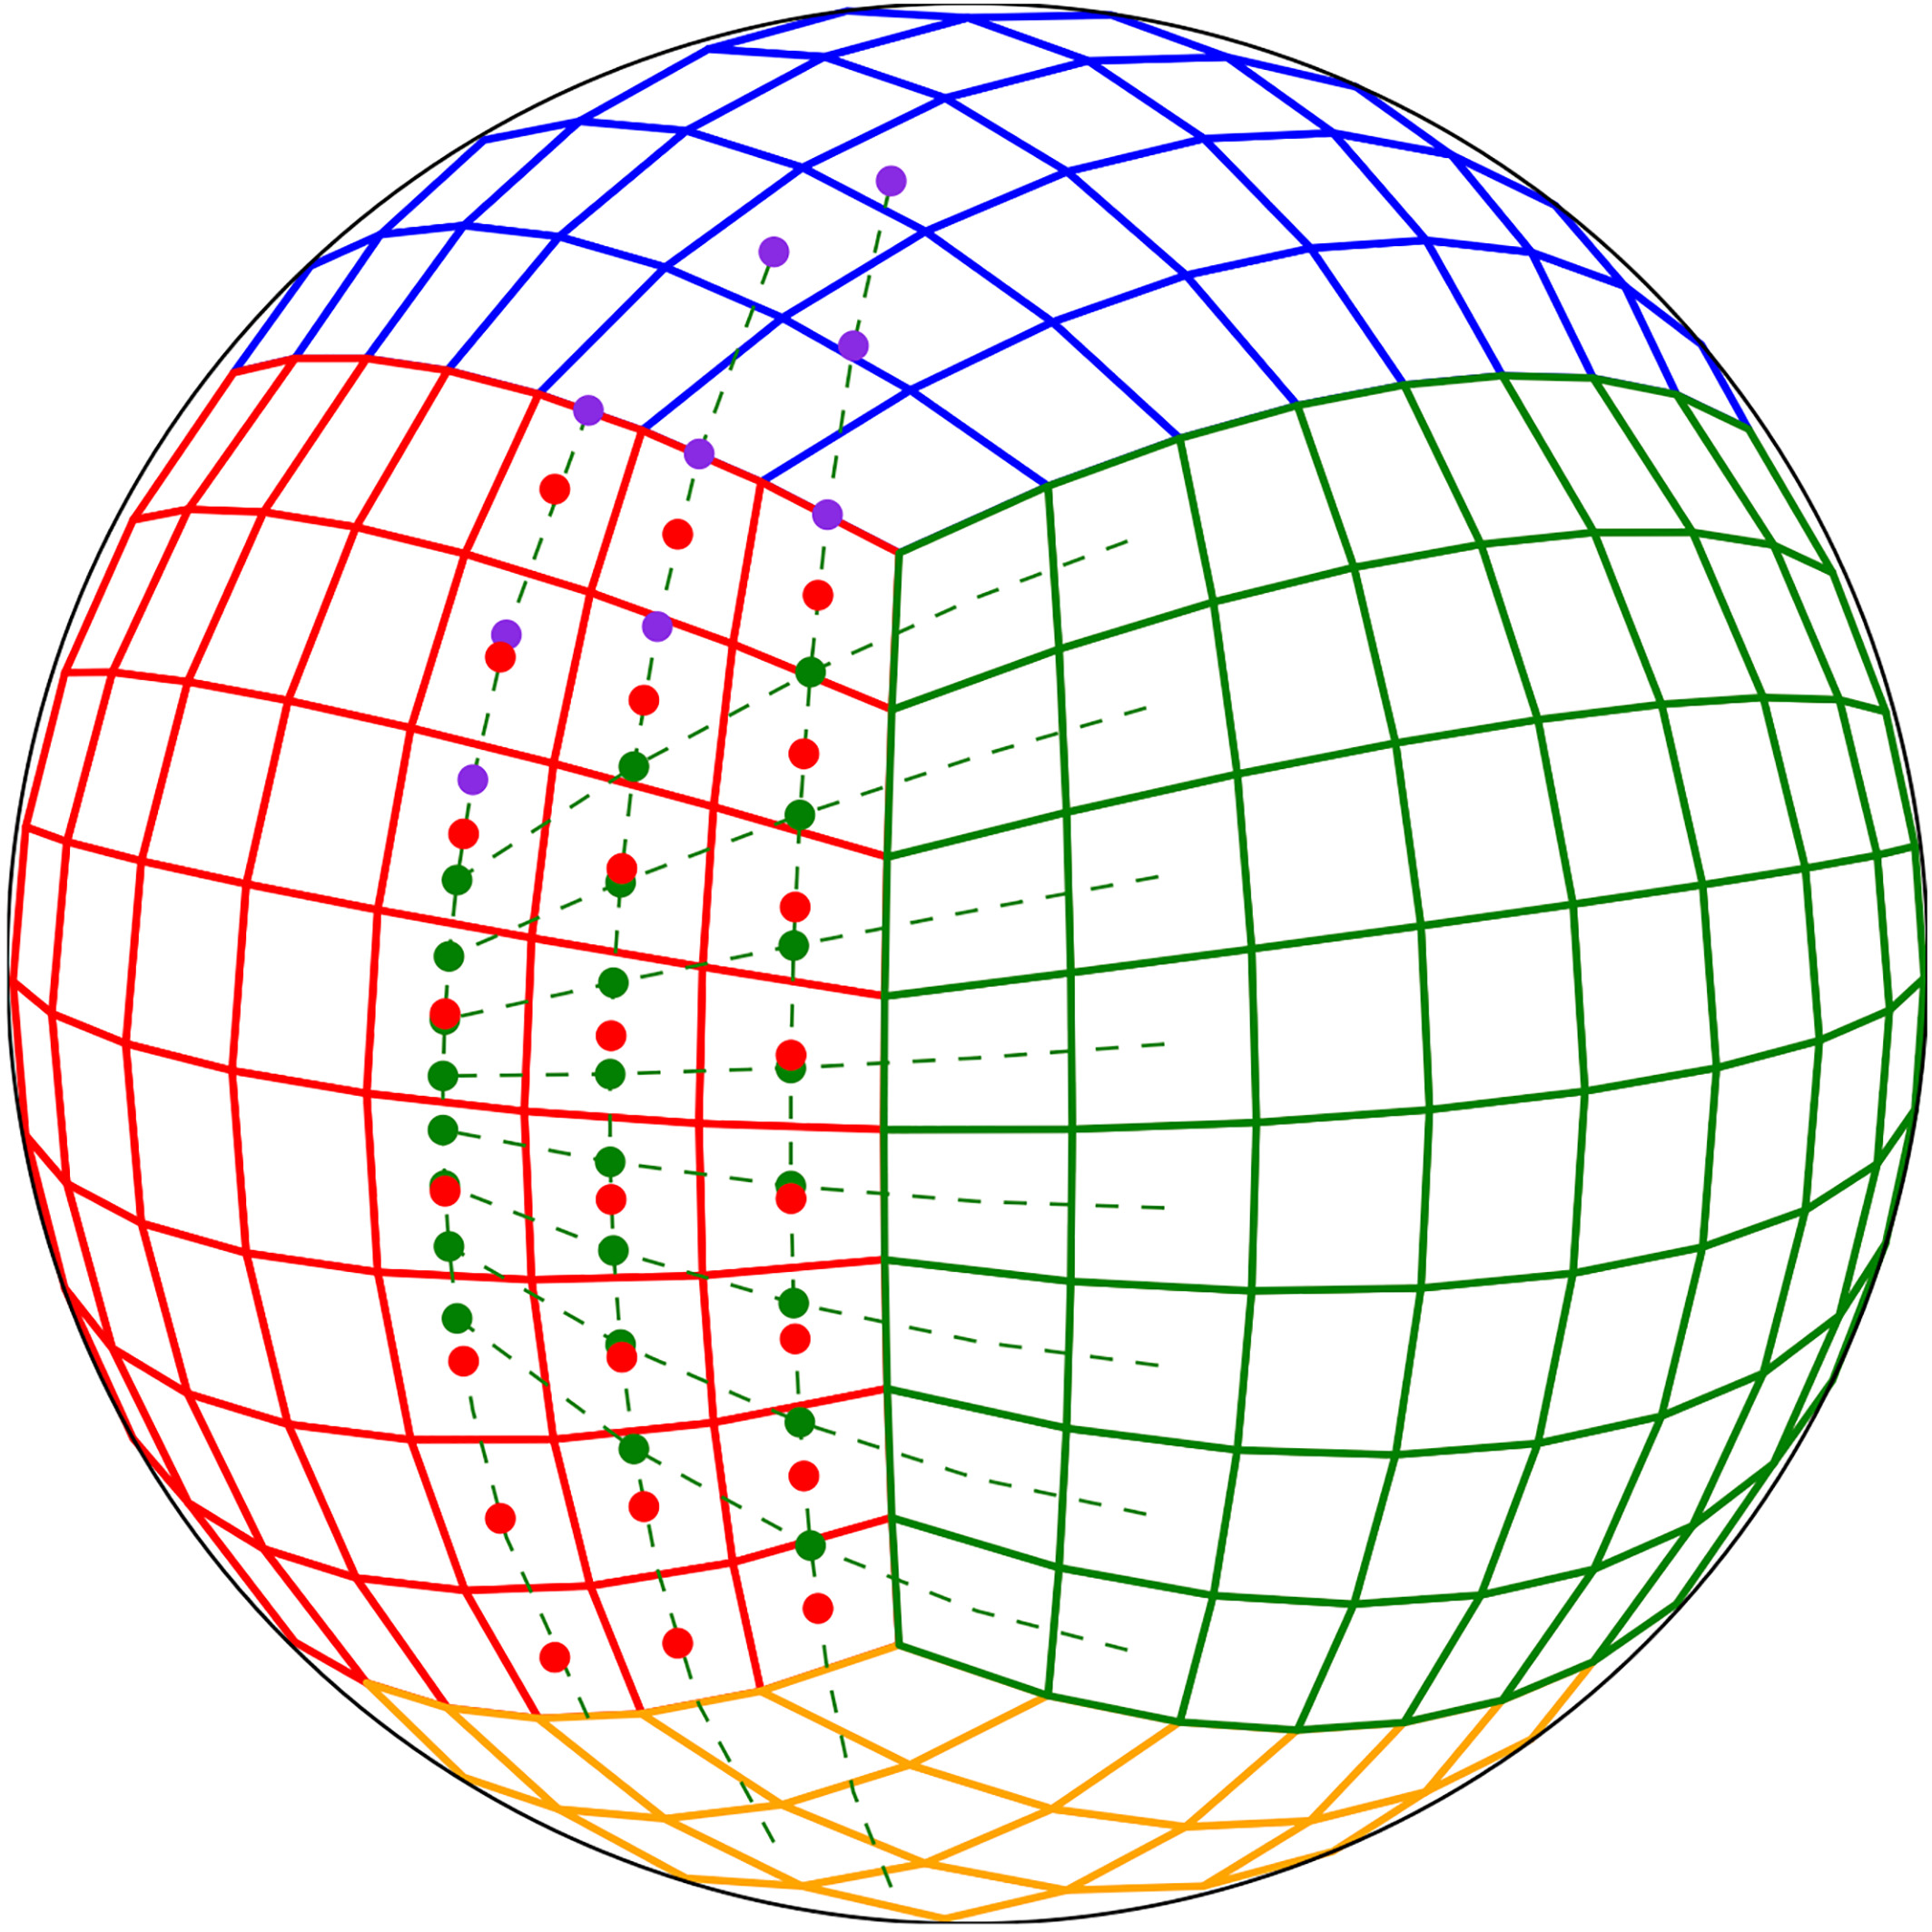
\includegraphics[width = 0.4\linewidth]{lagrange}
	\caption{Ghost cells on the equiangular cubed-sphere. Figure from \citet{chen:2021}}
	\label{lagrange}
\end{figure}

We adopted the strategy proposed by \citet{chen:2021},
that works only in the equiangular cubed-sphere.
This approach exploits that the center of the ghost cells
lye on a geodesic that connects the center of cells of the neighbor panel,
as it is shown in Figure \ref{lagrange}.
Therefore, we can employ a Lagrange interpolation over a geodesic
to approximate the values at the ghost cells.
We decided to use a third-order Lagrange interpolation.

\section{Numerical experiments}
We are going to show some results using the velocity vector field from
the deformational flow test case on the proposed by \citet{nair:2010}. 
In these simulation, we do not use the monotonicity constraints.

For the first test case, we assume that the scalar field $q$ is constant and equal to 1.
Since the velocity field is non-divergente, the scalar field should remain constant.


